%UNIT 16: Introduction to Laplace Transforms
%%%%%%%%%%%%%%%%%%%%%%%%%%%
%%%% Put the following at the top of each .tex file  %
\pagestyle{fancy}
\renewcommand{\theUnit}{6.1-6.2}
\ifthenelse{\isundefined{\UnitPageNumbers}}{}{\setcounter{page}{1}}
\rhead{Sections \theUnit: Properties of Laplace Transforms}
\lhead{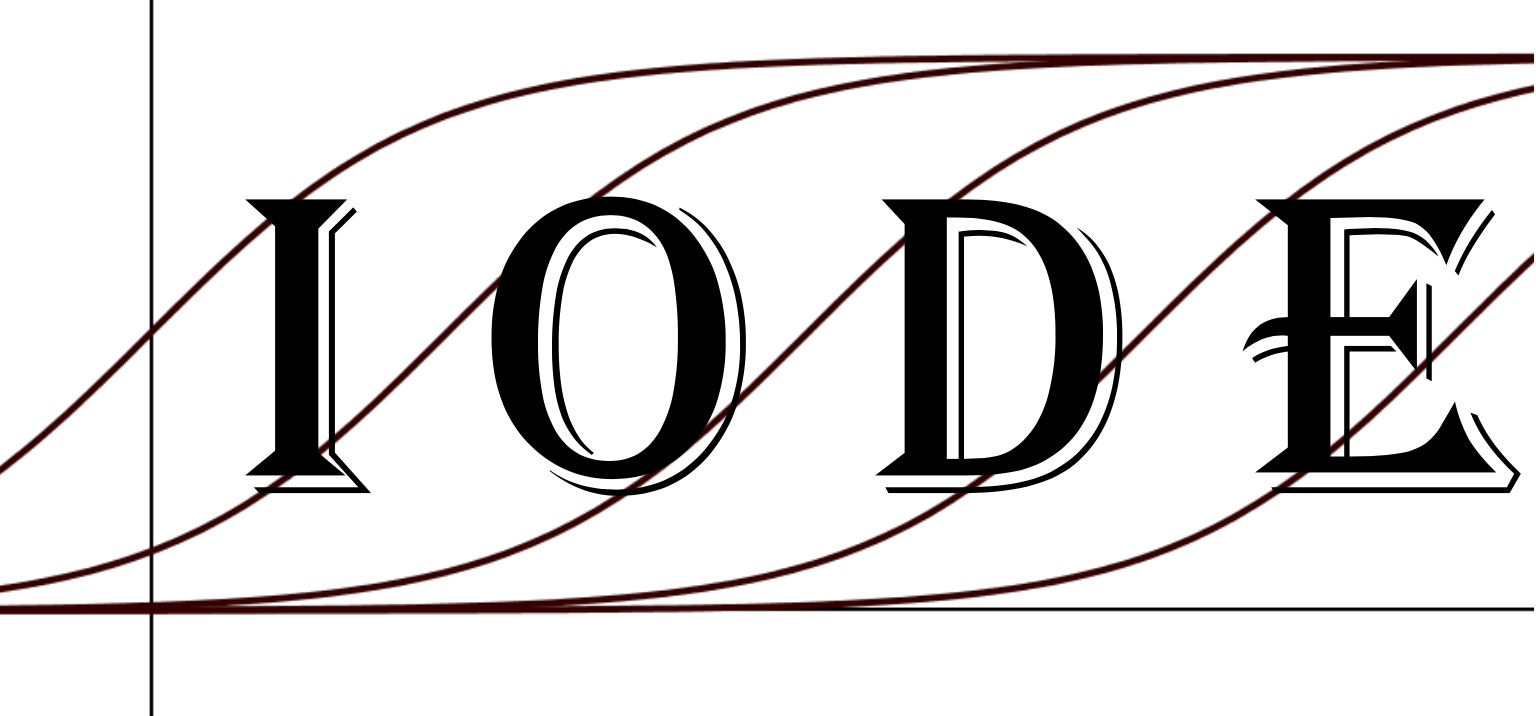
\includegraphics[width=1.25cm]{IODE-logo.png}}
\rfoot{\mypage}
\lfoot{}
\cfoot{}
\fancypagestyle{firstfooter}{\footskip = 50pt}
\renewcommand{\footrulewidth}{.4pt}
%%%%%%%%%%%%%%%%%%%%%%%%%%%
\vspace*{-20pt} \thispagestyle{firstfooter}
\pagebegin{Properties of the Laplace Transform}

\bb
\ii Let $f$, $f_1$, and $f_2$ be functions whose Laplace transform exists for $s > \alpha$ and let $c$ be a constant. Then for $s > \alpha$, prove the following:
\bb
\ii $\Lap \left\{ f_1 + f_2 \right\} = \Lap \left\{ f_1 \right\} + \Lap \left\{ f_2 \right\}$. \vfill
\ii $\Lap \left\{ cf \right\} = c \Lap \left\{ f \right\}$. \vfill
\ee
\ee


\clearpage

\pagebegin{Laplace Transform of  $g(t)=e^{at}f(t)$}

\begin{enumerate}
\ii If the Laplace transform $\mathscr{L}\{ f \} (s)=F(s)$ exist for $s > \alpha$, then show that
\[ \mathscr{L}\{ e^{at}f(t) \}= F(s-a), \ \ \mbox{for } s > \alpha + a.\]

\vfill

\ii Using the property above and the fact that $\mathscr{L} \{ \cos{(bt)} \} = \frac{s}{s^2+b^2}$ for $s >0$, find
$\Lap \{ e^{at} \cos{(bt)} \}$.

\vfill

\end{enumerate}

\clearpage

\pagebegin{Section 6.2: Laplace Transform of Derivatives }

\bbox
A function is of \textbf{exponential order} $\alpha$ if there exists positive constants $C$ and $T$ such that
\[ \left| f(t) \right| < Ce^{\alpha t} \ \ \mbox{for all } t > T.\]
For example:
\bi
\ii $f(t) = \cos{(5t)}e^{7t}$ has $\alpha = 7$.
\ii $e^{t^2}$ does not have an exponential order.
\ei
\ebox

\begin{enumerate}[resume]
\ii If $f(t)$ is continuous on $\lbrack 0, \infty )$ and $f'(t)$ is piecewise continuous on $\lbrack 0, \infty )$ with
both exponential order $\alpha$, then prove for $s > \alpha$,
\[ \mathscr{L} \{ f' \} = s \mathscr{L}\{ f \} - f(0) = sF(s)-f(0).\] \label{derprop}

\vfill

\clearpage

\ii Using the property from problem \ref{derprop} and the fact that $\mathscr{L} \{ \cos{(bt)} \} = \frac{s}{s^2+b^2}$ for $s >0$, find
$\Lap \{ \sin{(bt)} \}$. \vfill

\ii If $\Lap \{ f(t) \} = F(s)$ for all $s > \alpha$, using the property from problem \ref{derprop}, show that
\[ \Lap \{ f''(t) \} =s^2F(s)-sf(0)-f'(0) \quad \mbox{for all } s > \alpha .\]  \vfill
%by induction that $\Lap \{ t^n \} = \frac{n!}{s^{n+1}}$ for $s >0$.


\ii Using induction show that
\[ \Lap \{ f^{(n)} \} = s^n \Lap \{ f \} - s^{n-1} f(0) - s^{n-2} f'(0) - \ldots - f^{(n-1)}(0).\] \bs

\clearpage

\ii Let $F(s) = \Lap \{ f \}$ and assume $f(t)$ is piecewise continuous on $\lbrack 0, \infty )$ and of exponential order $\alpha$.
Prove that for $s > \alpha$ if follows that
\[ \Lap \{ t^nf(t) \} = (-1)^n \frac{d^nF}{ds^n}.\] \vfill


%\begin{example}
%Show by induction that $\Lap \{ t^n \} = \frac{n!}{s^{n+1}}$ for $s >0$.
\ii Using the definition of the Laplace transform, the result that $\Lap \{ e^{at} \} = \frac{1}{s-a}$ for $s>a$ and the property above, find a formula for  $\Lap \{ t^n e^{at} \}$. \vfill
%\end{example}
\end{enumerate}

\clearpage

\pagebegin{Common Laplace Transforms}

\begin{center}
\begin{tabular}{|l|l|}
\hline
$f(t)$ & $F(s) = \Lap \left\{ f(t) \right\}$ \\
\hline
$1$ & $\dsty \frac{1}{s}, \ s > 0$\\
\hline
$e^{at}$ & $\dsty \frac{1}{s-a}, \ s > a$\\
\hline
$t^n, \ n=1,2, \ldots$ & $\dsty \frac{n!}{s^{n+1}}, \ s > 0$\\
\hline
$\sin{(bt)}$ & $\dsty \frac{b}{s^2+b^2}, \ s > 0$\\
\hline
$\cos{(bt)}$ & $\dsty \frac{s}{s^2+b^2}, \ s > 0$\\
\hline
$e^{at}t^n, \ n=1,2, \ldots$ & $\dsty \frac{n!}{(s-a)^{n+1}}, \ s > a$\\
\hline
$e^{at}\sin{(bt)}$ & $\dsty \frac{b}{(s-a)^2+b^2}, \ s > a$\\
\hline
$e^{at}\cos{(bt)}$ & $\dsty \frac{s-a}{(s-a)^2+b^2}, \ s > a$\\
\hline
\end{tabular}
\end{center}
'
\bs

\pagebegin{Common Properties of Laplace Transforms}

\begin{enumerate}[label=L.\arabic*]
\ii $\mathscr{L} \left\{ cf(t) \right\} = c  \mathscr{L} \left\{ f(t) \right\}$, where $c$ is a constant. \ms

\ii $\mathscr{L} \left\{ f_1(t) + f_2(t) \right\} = \mathscr{L} \left\{ f_1(t) \right\} + \mathscr{L} \left\{ f_2(t)\right\}$ \ms

\ii If $F(s) = \mathscr{L} \left\{ f(t) \right\}$ exists for all $s > \alpha$, then $\dsty \mathscr{L} \left\{ e^{at} f(t) \right\} = F(s-a)$ for all $s>\alpha + a$.  \ms

\ii If $F(s) =\mathscr{L} \left\{ f(t) \right\}$ exists for all $s > \alpha$, then for all $s>\alpha$,
\[ \mathscr{L} \left\{ f^{(n)}(t) \right\} = s^n \mathscr{L} \{ f(t) \}-s^{n-1} f(0)- s^{n-2} f'(0) - \ldots - f^{(n-1)}(0).\] \ms

%\ii If $F(s) =\mathscr{L} \left\{ f(t) \right\}$ exists for all $s > \alpha$, then $\dsty \mathscr{L} \left\{ f'(t) \right\} = sF(s) -f(0)$ for all $s > \alpha$.
%\ii If $F(s) =\mathscr{L} \left\{ f(t) \right\}$ exists for all $s > \alpha$, then $\dsty \mathscr{L} \left\{ f''(t) \right\} = s^2 F(s) - sf(0)- f'(0)$ for all $s > \alpha$.

\ii If $F(s) =\mathscr{L} \left\{ f(t) \right\}$ exists for all $s > \alpha$, then $\dsty \mathscr{L} \left\{ t^n f(t) \right\} = (-1)^n \frac{d^nF}{ds^n}$ for all $s > \alpha$.
\ee


%\end{document}

%\begin{center}
%\begin{tabular}{|l|l|}
%\hline
%$f(t)$ & $F(s) = \Lap \left\{ f \right\} (s)$ \\
%\hline
%$1$ & $\dsty \frac{1}{s}, \ s > 0$\\
%\hline
%$e^{at}$ & $\dsty \frac{1}{s-a}, \ s > a$\\
%\hline
%$t^n, \ n=1,2, \ldots$ & $\dsty \frac{n!}{s^{n+1}}, \ s > 0$\\
%\hline
%$\sin{(bt)}$ & $\dsty \frac{b}{s^2+b^2}, \ s > 0$\\
%\hline
%$\cos{(bt)}$ & $\dsty \frac{s}{s^2+b^2}, \ s > 0$\\
%\hline
%$e^{at}t^n, \ n=1,2, \ldots$ & $\dsty \frac{n!}{(s-a)^{n+1}}, \ s > a$\\
%\hline
%$e^{at}\sin{(bt)}$ & $\dsty \frac{b}{(s-a)^2+b^2}, \ s > a$\\
%\hline
%$e^{at}\cos{(bt)}$ & $\dsty \frac{s-a}{(s-a)^2+b^2}, \ s > a$\\
%\hline
%\end{tabular}
%\end{center}


%A function is of \textbf{exponential order} $\alpha$ if there exists positive constants $C$ and $T$ such that
%\[ \left| f(t) \right| < Ce^{\alpha t} \ \ \mbox{for all } t > T.\]

%For example:
%\bi
%\ii $f(t) = \cos{5t}e^{7t}$ has $\alpha = 7$.
%\ii $e^{t^2}$ does not have an exponential order.
%\ei



